\documentclass{article}
\usepackage{tenor2015}
\usepackage{times}
\usepackage{ifpdf}
\usepackage[english]{babel}
\usepackage{cite}

\usepackage{listings}
\lstset{language=Python,
showspaces=false,
showtabs=false,
breaklines=false,
showstringspaces=false,
breakatwhitespace=false,
escapeinside={(*@}{@*)},
keywordstyle=\bfseries,
basicstyle=\scriptsize\ttfamily
}

\def\papertitle{Abjad, A Python API for Formalized Score Control}
\def\firstauthor{Trevor Ba\v{c}a}
\def\secondauthor{Josiah Wolf Oberholtzer}
\def\thirdauthor{Jeffrey Trevi\~{n}o}
\def\fourthauthor{Victor Ad\'{a}n}

\newif\ifpdf
\ifx\pdfoutput\relax
\else
   \ifcase\pdfoutput
      \pdffalse
   \else
      \pdftrue
\fi

\ifpdf % compiling with pdflatex
  \usepackage[pdftex,
    pdftitle={\papertitle},
    pdfauthor={\firstauthor, \secondauthor, \thirdauthor, \fourthauthor},
    bookmarksnumbered, % use section numbers with bookmarks
    pdfstartview=XYZ % start with zoom=100% instead of full screen; 
                     % especially useful if working with a big screen :-)
   ]{hyperref}
  %\pdfcompresslevel=9

  \usepackage[pdftex]{graphicx}
  % declare the path(s) where your graphic files are and their extensions so 
  %you won't have to specify these with every instance of \includegraphics
  \graphicspath{{./figures/}}
  \DeclareGraphicsExtensions{.pdf,.jpeg,.png}

  \usepackage[figure,table]{hypcap}

\else % compiling with latex
  \usepackage[dvips,
    bookmarksnumbered, % use section numbers with bookmarks
    pdfstartview=XYZ % start with zoom=100% instead of full screen
  ]{hyperref}  % hyperrefs are active in the pdf file after conversion
  \usepackage[dvips]{epsfig,graphicx}
  \graphicspath{{./figures/}}
  \DeclareGraphicsExtensions{.eps}
  \usepackage[figure,table]{hypcap}
\fi

\hypersetup{
    colorlinks,
    citecolor=black,
    filecolor=black,
    linkcolor=black,
    urlcolor=black
}

\title{\papertitle}

\fourauthors
  {\firstauthor} {Harvard \\
    {\tt \href{mailto:trevorbaca@gmail.com}
        {trevorbaca@gmail.com}}}
  {\secondauthor} {Harvard \\
    {\tt \href{mailto:josiah.oberholtzer@gmail.com}
        {josiah.oberholtzer@gmail.com}}}
  {\thirdauthor} { Carleton College \\
    {\tt \href{mailto:jeffrey.trevino@gmail.com}
        {jeffrey.trevino@gmail.com}}}
  {\fourthauthor} { Bank of America \\
    {\tt \href{mailto:vctradn@gmail.com}
        {vctradn@gmail.com}}}

\begin{document}

\capstartfalse
\maketitle
\capstarttrue

\begin{abstract}
Place your abstract at the top left column on the first page. Please write
about 150-200 words that specifically highlight the purpose of your work, its
context, and provide a brief synopsis of your results. Avoid equations in this
part.
\end{abstract}

\section{Introduction}\label{sec:introduction}

\begin{comment}
1. Changed "composers, music theorists and musicologists" to just "composers". How do we feel about this?
\end{comment}

Abjad\footnote{www.projectabjad.org} is an interactive software system designed
to help composers build up complex pieces of music notation in an iterative and
incremental way. Abjad is implemented in the Python\footnote{www.python.org}
programming language and architected as an object-oriented collection of
packages, classes and functions. Users can visualize their work as
publication-quality score at all stages of the compositional process using
Abjad's interface to the LilyPond\footnote{www.lilypond.org} music notation
package. Abjad is open-source software available for free download from the
Python Package Index.\footnote{pypi.python.org}

\begin{comment}
The current version of Abjad implements 491 public classes and 324 public
functions.
\end{comment}
\section{Background \& History}\label{sec:background}

\subsection{Composition as Notation}
While many environments for both notation and sound production have been authored within the last twenty years, the following discussion focuses solely on the production of notation: Abjad enables composers to express both low- and high-level compositional ideas by extending a widely used programming language to provide a sufficiently detailed object model of common practice musical notation. To minimize the restriction of artistic thought's infinite possibility while maximizing the ability to specify elegantly any arbitrary symbolic relationship, Abjad does this without prescribing explicit or implicit models of music or composition: Abjad defines composition narrowly as the act of creating a document via the encoded aggregation of notational symbols.

\subsection{Computational Models of Notation}

Many systems implement detailed models of music explicitly or implicitly, but few of these implement detailed models of notation.\footnote{Computational models of music might entail the representation of higher-level musical entities apparent in the acts of listening and analysis but absent in the symbols of notation themselves, as determined to be creatively exigent. Programming researchers and musical artists have modeled many such extrasymbolic musical entities, such as large-scale form and transition \cite{polansky1991morphological}, \cite{uno1994temporal}, \cite{dobrian1995algorithmic}, \cite{abrams1999higher}, \cite{Yoo1983}, texture \cite{Horenstein:2004kx}, contrapuntal relationships \cite{Boenn:2009oq}, \cite{Acevedo2005}, \cite{Anders:2011kl}, \cite{Balser:1990tg}, \cite{Jones:2000hc}, \cite{uno1994temporal}, \cite{Bell:1995ij}, \cite{farbood2001analysis}, \cite{Cope:2002fv}, \cite{Laurson:2005dz}, \cite{Polansky:2011fu}, \cite{Ebcioglu:1980kl}, harmonic tension and resolution \cite{Melo2003}, \cite{Wiggins1999}, \cite{Foster:1995qa}, melody \cite{Hornel:1993mi}, \cite{Smith:1992pi}, meter \cite{Hamanaka:2005ff}, rhythm \cite{Nauert2007}, \cite{Degazio:1996lh}, \cite{Collins:2003bs}, timbre \cite{Xenakis:1991fu}, \cite{Creasey:1996ye}, \cite{Osaka2004}, temperament \cite{Seymour:2007qo}, \cite{Graf:2006il}, and ornamentation \cite{Ariza:2003zt}, \cite{Chico-Topfer:1998jl}. This work overlaps fruitfully with analysis tasks, and models of listening and cognition can enable novel methods of high-level musical structures and transformations, like dramatic direction, tension, and transition between sections \cite[108]{Collins2009}.} A system that affords a detailed model of music/composition without linking to a sufficiently detailed model of musical notation does not afford automated notation --- sufficiency, however, depends heavily on generative task. For example, if a composer requires an automated notation system to render complex rhythmic ideas that depend typographically on nested tuplets, a system that produces a notation only via a combination of MIDI and quantization must reduce rhythms to a non-hierarchical stream of event times, eliminating the temporally divisive approach of tuplet notation. For many rhythmic applications, though, MIDI suffices. 

Many automated notation systems exist to model musical notation and the act of typographical layout without explicitly affording the computational modeling of music or composition \cite{Smith:1972mw}, \cite{Nienhuys:2003ve}, \cite{Hoos:1998bd}, \cite{hamel1noteability}; many of these systems strongly imply a model of music, such as Gr\'{e}goire for Gregorian chant, Django for guitar tablature, and GOODFEEL for Braille notation \cite{2006}. In this light, feature-rich systems oriented toward classical composers, such as Finale, Sibelius, SCORE, Igor, Berlioz, and Nightingale fit into the mold of systems that model notation with genre as a primary determinant of generative task. Such a system might go so far as to enable a text-based object-oriented model of notation that automates some aspect of an otherwise point-and-click interface, as in the case of Sibelius's ManuScript scripting language \cite{Technology:qc}. 

Many models of musical notation were created for purposes of corpus-based computational musicology. Formats such as Music21, DARM, SMDL, HumDrum, and MuseData model notation with the generative task of searching through a large amount of data \cite{Selfridge-Field:1997ud}. Commercial notation software developers attempted to establish a data interchange standard for optical score recognition (NIFF) \cite{niff1995niff}; since its release in 2004, MusicXML has become a valid interchange format for over 160 applications and maintains a relatively application-agnostic status, as it was designed with the generative task of acting as an interchange format between variously tasked systems \cite{Good:2001if}. (are Igor and Berlioz commercial?)

Notation representations that underly many of these GUI-based systems often go undescribed as computer representations of notation, in favor of discussions about human-computer interaction. For example, Barker and Cantor developed an early model of music notation that underlies a four-oscilloscope GUI and describe their work entirely in terms of user interaction \cite{cantor1971computer}; likewise, discussions of modern commercial notation systems remain similarly oriented, without much awareness or criticism of the underlying computational models of notation. This results in insufficiently detailed models of notation; systems, for example, that provide models only of mensural notation and enable nonmensural notations only as modified instantiations of notations based on measures.

\subsection{The Development of Hierarchical Object Models of Notation}
Many early models of musical notation were not hierarchical, and Lejaran Hiller, in reflecting on decades of automated notation work, identifies the lack of hierarchical organization as a limitation of early work --- although Nick Collins points out that even Hiller's program PHRASE addresses the hierarchical organization of a score up to the level of a phrase, without moving beyond this mid-level musical structure to concerns of large-scale form \cite[108]{Collins2009}. 

There were several object-oriented music environments by 1990 \cite[139]{Polansky:1990fk}, most created in or inspired by the newly popular Smalltalk-80 programming language; while they facilitated the hierarchical modeling of musical abstractions, they omitted or radically simplified the hierarchical nature of common notation. For example, Glen Krasner (Xerox Systems Science Laboratory) created Machine Tongues VIII, a music system that created an object-oriented model of the score/orchestra distinction inherited from Max Mathews' Music N languages, with a simple linear model of ``partOn'' and ``partOff'' command sequences \cite{Krasner:1991uq}, omitting hierarchical organization entirely when the system produced notational output; although subsequent Machine Tongues systems introduced some hierarchical organization via ``note'' objects that inhabited ``event lists,'' systems did not attempt to model the hierarchical detail of all a traditional score's elements. Like Hiller's PHRASE program, Andreas Mahling's CompAss system organized events hierarchically up to the mid-level ``phrase'' level of musical structure \cite{Mahling:1991qf}. These systems extend Smalltalk-80 with interfaces to the MIDI communications protocol: as extensions of Smalltalk, they enabled the user to arbitrarily extend the system with new objects, creating a detailed and hierarchical model of music, usually flattened into a list of noteOn and noteOff commands to be notated or played back via MIDI interface. 

By 1989, Glendon Diener's Nutation system (written in Objective C for the NeXT computer) modeled both musical and notational structure hierarchically through the use of directed graphs \cite{Diener:1991zr}, \cite{Diener:1991ly}, \cite{Diener:1989ve}.

last section: system motivations
	

Linking our design priorities with those of previous systems by describing perceived deficiencies: evaluative priorities for previous systems: sufficiency instead of comprehensiveness, potentially evaluated by sonic result rather than notation, addressability (in HMSL and JMSL). Reintroduce generative task: late 50s through 80s were motivated locally by generative tasks of specific projects until IRCAM's Patchwork approached a generative task of broadly enabling composers; sufficiency determined by comprehensive task.
\section{Notational isomorphism}\label{sec:notational_isomorphism}

\subsection{Notational aggregation}

Abjad models objects on the page according to common practice notation. Abjad
assumes notational primitives are the elements of composition. The act of
composition then revolves around the iterative aggregation of notational
primitives into arbitrarily complex score objects.

Abjad allows for the iterative aggregation of notational elements via Python's
\emph{mutable sequence} protocol. Score components can be appended, extended or
inserted into other container-like score components.

\begin{lstlisting}
>>> score = Score()
>>> staff_group = StaffGroup()
>>> upper_staff = Staff()
>>> lower_staff = Staff()
>>> score.append(staff_group)
>>> staff_group.extend([upper_staff, lower_staff])
>>> upper_staff.extend("c'4 d'4 e'4 f'4")
>>> lower_staff.extend([Chord("<a ef'>4."), Note("g8")])
>>> lower_staff.insert(0, Rest((1, 2)))
>>> show(score)
\end{lstlisting}

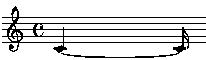
\includegraphics[scale=1.0]{images/section_2_notational_isomorphism-1.pdf}


Note that Abjad makes visualizing notational artifacts simple. Any notational
element or aggregate can be displayed at any time as a PDF via calls to its
top-level \texttt{show()} function in publication quality.

Spanners such as slurs, beams and glissandi and indicators such as
articulations and textual directions can be attached to score components via
the \texttt{attach()} function.

\begin{lstlisting}
>>> attach(Slur(), upper_staff[:])
>>> attach(Glissando(), lower_staff[1:])
>>> attach(Articulation('accent'), lower_staff[-1])
>>> show(score)
\end{lstlisting}

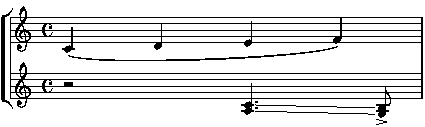
\includegraphics[scale=1.0]{images/section_2_notational_isomorphism-2.pdf}


Abjad attempts to be compositionally agnostic. By providing simple and
unambiguous means of gradually aggregating arbitrarily complex score objects,
Abjad encourages users to develop their own personal approach.

\subsection{Explicit notational modeling}

Abjad models notation explicitly. All notational primitives expressed by Abjad
must conform to the principles of common practice notation. When compositional
inputs cannot be expressed in terms of these principles, Abjad provides
affordances for massaging them into valid notational states.

For example, Abjad expresses the durations of all score components in terms of
rational values -- fractions and integers -- rather than floating point
numbers. Likewise Abjad expresses all pitches in terms of triples of diatonic
note names, accidentals and octave numbers, rather than MIDI numbers or
frequencies. While Abjad provides alternative representations of pitch and
rhythm, as well as affordances for moving between them, the format actually
stored in and used by score components for rendering notation is always the
most notationally-explicit.

\subsection{Written, assignable and prolated durations}

All \texttt{Note}, \texttt{Chord} and \texttt{Rest} objects in Abjad must be
instantiated with a duration corresponding to the written glyphs on the page --
a \emph{written} duration.

Written durations must be \emph{assignable}, a category we invented to model
durational initialization. Durational assignability describes whether a
duration can be represented as a power-of-two flag count combined with zero or
more dots. \texttt{1/4}, \texttt{3/16} and \texttt{7/16} are assignable
durations while \texttt{5/32}, \texttt{9/8} and \texttt{1/12} are not.

Non-assignable durations cannot be represented in common practice notation by a
single glyph. They require two or more glyphs with assignable durations tied
together, for the score component to be tupletted, or both.

Abjad will not automatically render a single note with a duration of
\texttt{5/16} as two or more notes tied together. We consider such behavior to
be too implicit. There are too many potentially compositionally valid ways to
render a duration such as \texttt{5/16} into a series of tied assignable
durations: \texttt{1/4 + 1/16}, \texttt{3/16 + 2/16}, \texttt{2/16 + 3/16},
\texttt{1/16 + 1/4}, \texttt{1/8 + 1/8 + 1/16} etc. Instead we provide
affordances for generating tied notes from non-assignable durations. One such
affordance is our \texttt{scoretools.make\_notes()} function, which chooses
smart defaults for generating tied glyphs from otherwise un-notateable input.

\begin{lstlisting}
>>> selection = scoretools.make_notes("c'", [(5, 16)])
>>> staff = Staff(selection)
>>> show(staff)
\end{lstlisting}

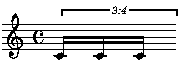
\includegraphics[scale=1.0]{images/section_2_notational_isomorphism-3.pdf}


All score components also have a \emph{prolated} duration - the product of
their written duration and their \emph{prolation}. Prolation is the cumulative
product of all the \emph{multiplier} of every tuplet found in the
\emph{parentage} of a score component. A score component's prolation depends on
its location in the score hierarchy, and is not an inherent property of itself
independent that hierarchy.

Three \texttt{Note} objects each having a prolated duration of \texttt{1/12}
can be represented as either three \texttt{1/16} notes in a \texttt{3:4} tuplet
or as three \texttt{1/8} notes in a \texttt{3:2} tuplet. As all Abjad
\texttt{Note} objects must have an assignable written duration, the three notes
above must have written durations of either \texttt{1/8} or \texttt{1/16}, and
the tuplet must be correspondingly an explicit diminution or augmentation to
provide the desired prolation of \texttt{2/3} or \texttt{4/3}.

\begin{lstlisting}
>>> selection = scoretools.make_notes("c'", [(1, 12)] * 3)
>>> tuplet = selection[0]
>>> show(tuplet)
\end{lstlisting}

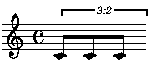
\includegraphics[scale=1.0]{images/section_2_notational_isomorphism-4.pdf}

\begin{lstlisting}
>>> tuplet.toggle_prolation()
>>> show(tuplet)
\end{lstlisting}

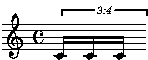
\includegraphics[scale=1.0]{images/section_2_notational_isomorphism-5.pdf}


The durational information of any aggregate score object in Abjad is therefore
always explicit and unambiguous with regard to its notational reality.
\section{Relationship Modeling}\label{sec:relationship_modeling}

\subsection{Component, Spanner, Indicator}

Graph-theoretic relationships

Attachment relationships

Selections

Bidirectional vs unidirectional pointers.

Indicator scope

\subsection{Timespans}

A \emph{timespan} is an object-oriented model of a start/stop offset pair.
Abjad's \texttt{Timespan} class affords users with a variety of tests for
relationships between timespans such as overlap and intersection.

All durated objects in Abjad have a timespan, including all score components
and spanners, allowing them to partake in timespan-based relationship modeling
without regard for hierarchical score structure.
\section{Score Addressibility}\label{sec:score_addressability}
\section{Extensibility}\label{sec:extensibility}
\subsection{Compositional Agnosticism}
     By providing core functionality oriented toward the elements of standard notation, Abjad strives to remain as agnostic as possible to various composition techniques. 
\subsection{Example Extensions}
To better afford high-level, personal, eccentric composition techniques as optional tools packages, Abjad provides clear examples of extensibility through the authors' own included extensions, including: 
        - labeltools
        - metertools
        - quantizationtools
        - rhythmmakertools
        - selectortools
        - sievetools
        - tonalanalysistools
\subsection{Affording Extension through Project Structure and Interface}
As an open-source project, composers and researchers can contribute changes via git pull requests. A process of continuous integration and online version control simplifies this contribution process. 

\section{Embeddability}\label{sec:embeddability}

Abjad is an importable Python library. It can be used in whole or in part as a
component of any Python-compatible system. Abjad has few Python package
dependencies and is not bound to any specific user application or graphic user
interface. These qualities make Abjad an ideal project ideal for embedding in
other software systems.

For example, Abjad supports IPython
Notebook\footnote{http://ipython.org/notebook.html}, a web-based interactive
computational environment combining code execution, text, mathematics, plots
and rich media into a single document. Notational output from Abjad can
be transparently captured and embedded directly into an IPython Notebook which
has loaded Abjad's IPython Notebook extension.

\section{Open Source}\label{sec:open_source}

\begin{acknowledgments}
You may acknowledge people, projects, 
funding agencies, etc. 
which can be included after the second-level heading
``Acknowledgments'' (with no numbering).
\end{acknowledgments} 

\bibliography{tenor2015template}
\end{document}